
\subsection{Electrical Features NeuroElectro Experiment Features}

\begin{table}[ht]
\centering
\resizebox{\textwidth}{!}{
\begin{tabular}{lllll}
\toprule
name & Hippocampus CA1 pyramidal cell & Cerebellum Purkinje cell & Neocortex pyramidal cell layer 5-6 &      olfactory mitral cell \\ 
\midrule
RheobaseTest                   &                     189.24 pA &                680.79 pA &                          213.85 pA &          NaN \\
InputResistanceTest            &                    107.08 Mohm &              142.06 Mohm &                        120.67 Mohm &  130.08 Mohm \\
TimeConstantTest               &                        24.5 ms &                      NaN &                           15.73 ms &     24.48 ms \\
CapacitanceTest                &                        89.8 pF &                620.27 pF &                          150.58 pF &    235.75 pF \\
RestingPotentialTest           &                      -65.23 mV &                -61.59 mV &                          -68.25 mV &    -58.14 mV \\
APWidthTest     &                        1.32 ms &                  0.41 ms &                            1.21 ms &      1.61 ms \\
APAmplitudeTest &                       86.36 mV &                 71.23 mV &                           80.44 mV &      68.4 mV \\
APThresholdTest &                       -47.6 mV &                -46.89 mV &                          -42.74 mV &     -38.9 mV \\
\bottomrule
\end{tabular}}
\end{table} 

\subsection{Agreement between Model and experiments:}
 \subsubsection{ Experiment: Neocortex pyramidal cell layer 5-6 Model:IZHikevich}

\begin{table}[ht]
\centering
\resizebox{\textwidth}{!}{
 \begin{tabular}{llll}
\toprule
{} &           observations &                 predictions &    Z-Scores \\
\midrule
RheobaseTest                   &    213.849583333333 pA &                   289.16 pA &    0.417618 \\
InputResistanceTest            &  120.672073643411 Mohm &  60.721628079999995 megaohm &    0.821026 \\
TimeConstantTest               &    15.7342424242424 ms &                     9.18 ms &    0.994512 \\
CapacitanceTest                &    150.584166666667 pF &                      0.0 pF &  0.00325377 \\
RestingPotentialTest           &   -68.2481434599156 mV &                   -66.08 mV &    0.300507 \\
InjectedCurrentAPWidthTest     &    1.20769387755102 ms &                      0.0 ms &     4.16142 \\
InjectedCurrentAPAmplitudeTest &    80.4351020408164 mV &                    80.52 mV &  0.00513793 \\
InjectedCurrentAPThresholdTest &   -42.7357232704403 mV &                   -43.97 mV &    0.130095 \\
\bottomrule

\end{tabular}}
\end{table} 

\begin{table}[ht]
\centering
\resizebox{\textwidth}{!}{
\begin{tabular}{llll}
\toprule
{} &           observations &                predictions &   Z-Scores \\
\midrule
RheobaseTest                   &              189.24 pA &                   32.24 pA &   0.536865 \\
InputResistanceTest            &  107.080327644332 Mohm &  97.76274731999999 megaohm &   0.100485 \\
TimeConstantTest               &    24.5021946169772 ms &                     9.6 ms &   0.717214 \\
CapacitanceTest                &    89.7960714285714 pF &                     0.0 pF &   0.133624 \\
RestingPotentialTest           &   -65.2261863636364 mV &                  -65.56 mV &  0.0554458 \\
InjectedCurrentAPWidthTest     &    1.31895278450363 ms &                     0.0 ms &    0.16846 \\
InjectedCurrentAPAmplitudeTest &     86.364525297619 mV &                   86.97 mV &  0.0399524 \\
InjectedCurrentAPThresholdTest &   -47.5985714285714 mV &                   -40.0 mV &    1.12315 \\
\bottomrule
\end{tabular}}
\end{table} 


\subsection{The Experimental Measurements}\begin{tabular}{lllll}
\toprule
name & Hippocampus CA1 pyramidal cell & Cerebellum Purkinje cell & Neocortex pyramidal cell layer 5-6 &      olf\_mit \\
\midrule
RheobaseTest                   &                      189.24 pA &                680.79 pA &                          213.85 pA &          NaN \\
InputResistanceTest            &                    107.08 Mohm &              142.06 Mohm &                        120.67 Mohm &  130.08 Mohm \\
TimeConstantTest               &                        24.5 ms &                      NaN &                           15.73 ms &     24.48 ms \\
CapacitanceTest                &                        89.8 pF &                620.27 pF &                          150.58 pF &    235.75 pF \\
RestingPotentialTest           &                      -65.23 mV &                -61.59 mV &                          -68.25 mV &    -58.14 mV \\
InjectedCurrentAPWidthTest     &                        1.32 ms &                  0.41 ms &                            1.21 ms &      1.61 ms \\
InjectedCurrentAPAmplitudeTest &                       86.36 mV &                 71.23 mV &                           80.44 mV &      68.4 mV \\
InjectedCurrentAPThresholdTest &                       -47.6 mV &                -46.89 mV &                          -42.74 mV &     -38.9 mV \\
\bottomrule
\end{tabular}
\subsection{Neocortex pyramidal cell layer 5-6, Izhikevich Model}\chi^{2}\begin{tabular}{lr}
\toprule
{} &         0 \\
\midrule
chi\_square &  1.976320 \\
p\_value    &  0.981729 \\
\bottomrule
\end{tabular}
\begin{tabular}{llll}
\toprule
{} &           observations &                predictions & Z-Scores \\
\midrule
RheobaseTest                   &    213.849583333333 pA &                   45.04 pA &     1.13 \\
InputResistanceTest            &  120.672073643411 Mohm &  84.47885606999999 megaohm &     0.44 \\
TimeConstantTest               &    15.7342424242424 ms &                   12.28 ms &     0.45 \\
CapacitanceTest                &    150.584166666667 pF &                     0.0 pF &     0.03 \\
RestingPotentialTest           &   -68.2481434599156 mV &                  -68.35 mV &     0.01 \\
InjectedCurrentAPWidthTest     &    1.20769387755102 ms &                     0.0 ms &     0.16 \\
InjectedCurrentAPAmplitudeTest &    80.4351020408164 mV &                    80.5 mV &        0 \\
InjectedCurrentAPThresholdTest &   -42.7357232704403 mV &                  -38.51 mV &     0.51 \\
\bottomrule
\end{tabular}
\subsection{Hippocampus CA1 pyramidal cell, Izhikevich Model}\chi^{2}\begin{tabular}{lrr}
\toprule
{} &  chi\_square &   p\_value \\
\midrule
0 &    2.125091 &  0.976935 \\
\bottomrule
\end{tabular}
\begin{tabular}{llll}
\toprule
{} &           observations &                predictions & Z-Scores \\
\midrule
RheobaseTest                   &              189.24 pA &                   32.24 pA &     0.54 \\
InputResistanceTest            &  107.080327644332 Mohm &  97.76274731999999 megaohm &      0.1 \\
TimeConstantTest               &    24.5021946169772 ms &                     9.6 ms &     0.72 \\
CapacitanceTest                &    89.7960714285714 pF &                     0.0 pF &     0.13 \\
RestingPotentialTest           &   -65.2261863636364 mV &                  -65.56 mV &     0.06 \\
InjectedCurrentAPWidthTest     &    1.31895278450363 ms &                     0.0 ms &     0.17 \\
InjectedCurrentAPAmplitudeTest &     86.364525297619 mV &                   86.97 mV &     0.04 \\
InjectedCurrentAPThresholdTest &   -47.5985714285714 mV &                   -40.0 mV &     1.12 \\
\bottomrule
\end{tabular}
\subsection{Hippocampus CA1 pyramidal cell, Conductance Model}\chi^{2}\begin{tabular}{lrr}
\toprule
{} &  chi\_square &   p\_value \\
\midrule
0 &   17.216463 &  0.027932 \\
\bottomrule
\end{tabular}
\begin{tabular}{llll}
\toprule
{} &           observations &           predictions & Z-Scores \\
\midrule
RheobaseTest                   &              189.24 pA &              225.0 pA &      0.1 \\
InputResistanceTest            &  107.080327644332 Mohm &  130.26055974 megaohm &     0.27 \\
TimeConstantTest               &    24.5021946169772 ms &               6.52 ms &     0.91 \\
CapacitanceTest                &    89.7960714285714 pF &                0.0 pF &     0.78 \\
RestingPotentialTest           &   -65.2261863636364 mV &             -63.79 mV &     0.26 \\
InjectedCurrentAPWidthTest     &    1.31895278450363 ms &                0.0 ms &     2.54 \\
InjectedCurrentAPAmplitudeTest &     86.364525297619 mV &              89.14 mV &      0.2 \\
InjectedCurrentAPThresholdTest &   -47.5985714285714 mV &             -62.83 mV &     3.02 \\
\bottomrule
\end{tabular}
\subsection{Hippocampus CA1 pyramidal cell, Adaptive Exponential Model}\chi^{2}\begin{tabular}{lr}
\toprule
{} &          0 \\
\midrule
chi\_square &  10.232514 \\
p\_value    &   0.249084 \\
\bottomrule
\end{tabular}
\begin{tabular}{llll}
\toprule
{} &           observations &           predictions & Z-Scores \\
\midrule
RheobaseTest                   &              189.24 pA &              225.0 pA &      0.1 \\
InputResistanceTest            &  107.080327644332 Mohm &  130.26055974 megaohm &     0.27 \\
TimeConstantTest               &    24.5021946169772 ms &               6.52 ms &     0.91 \\
CapacitanceTest                &    89.7960714285714 pF &                0.0 pF &     0.78 \\
RestingPotentialTest           &   -65.2261863636364 mV &             -63.79 mV &     0.26 \\
InjectedCurrentAPWidthTest     &    1.31895278450363 ms &                0.0 ms &     2.54 \\
InjectedCurrentAPAmplitudeTest &     86.364525297619 mV &              89.14 mV &      0.2 \\
InjectedCurrentAPThresholdTest &   -47.5985714285714 mV &             -62.83 mV &     3.02 \\
\bottomrule
\end{tabular}
\subsection{Olfactory Mitral Cell Izhikevich Model}\begin{tabular}{llll}
\toprule
{} &           observations &           predictions & Z-Scores \\
\midrule
InputResistanceTest            &  130.083333333333 Mohm &  111.76440601 megaohm &     0.21 \\
TimeConstantTest               &    24.4833333333333 ms &              26.35 ms &     0.18 \\
CapacitanceTest                &              235.75 pF &                0.0 pF &     0.03 \\
RestingPotentialTest           &          -58.140625 mV &             -59.78 mV &      0.3 \\
InjectedCurrentAPWidthTest     &                1.61 ms &                0.0 ms &     0.19 \\
InjectedCurrentAPAmplitudeTest &                68.4 mV &              68.62 mV &     0.04 \\
InjectedCurrentAPThresholdTest &               -38.9 mV &             -30.45 mV &     1.35 \\
\bottomrule
\end{tabular}
\subsubsection{Neocortex pyramidal cell layer 5-6ADEXP Model}\begin{tabular}{lr}
\toprule
{} &          0 \\
\midrule
chi\_square &  31.871046 \\
p\_value    &   0.000098 \\
\bottomrule
\end{tabular}
\begin{tabular}{llll}
\toprule
{} &           observations &          predictions & Z-Scores \\
\midrule
RheobaseTest                   &    213.849583333333 pA &            212.59 pA &     0.01 \\
InputResistanceTest            &  120.672073643411 Mohm &  80.93939761 megaohm &      0.5 \\
TimeConstantTest               &    15.7342424242424 ms &              9.91 ms &     0.85 \\
CapacitanceTest                &    150.584166666667 pF &               0.0 pF &     0.17 \\
RestingPotentialTest           &   -68.2481434599156 mV &            -66.93 mV &     0.17 \\
InjectedCurrentAPWidthTest     &    1.20769387755102 ms &               0.0 ms &     5.55 \\
InjectedCurrentAPAmplitudeTest &    80.4351020408164 mV &             80.72 mV &     0.02 \\
InjectedCurrentAPThresholdTest &   -42.7357232704403 mV &            -44.95 mV &     0.24 \\
\bottomrule
\end{tabular}


    \hypertarget{izhikevich-model-hippocampus-ca1-pyramidal-experiment.}{%
\section{Izhikevich model Hippocampus CA1 pyramidal
experiment.}\label{izhikevich-model-hippocampus-ca1-pyramidal-experiment.}}


        

    

    \begin{center}
    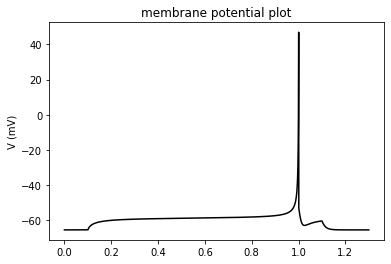
\includegraphics[]{notebooks_converted/make_normal_distribution_files/make_normal_distribution_8_2.png}
    \end{center}

    \hypertarget{conductance-based-model-hippocampus-ca1-pyramidal-experiment.}{%
\section{Conductance Based model Hippocampus CA1 pyramidal
experiment.}\label{conductance-based-model-hippocampus-ca1-pyramidal-experiment.}}

            \begin{tcolorbox}
            %[breakable, size=fbox, boxrule=.5pt, pad at break*=1mm, opacityfill=0]
\begin{Verbatim}[commandchars=\\\{\}]
   chi\_square   p\_value
0   17.216463  0.027932
\end{Verbatim}
\end{tcolorbox}
        
    

            \begin{tcolorbox}[breakable, size=fbox, boxrule=.5pt, pad at break*=1mm, opacityfill=0]
\begin{Verbatim}[commandchars=\\\{\}]
   chi\_square   p\_value
0   17.216463  0.027932
\end{Verbatim}
\end{tcolorbox}
        
            \begin{tcolorbox}[breakable, size=fbox, boxrule=.5pt, pad at break*=1mm, opacityfill=0]
\begin{Verbatim}[commandchars=\\\{\}]
   RheobaseTest  InputResistanceTest  TimeConstantTest  CapacitanceTest  \textbackslash{}
0      0.104364              0.26776          0.909698         0.779279

   RestingPotentialTest  InjectedCurrentAPWidthTest  \textbackslash{}
0              0.263258                    2.539904

   InjectedCurrentAPAmplitudeTest  InjectedCurrentAPThresholdTest
0                        0.197484                        3.023183
\end{Verbatim}
\end{tcolorbox}
        
            \begin{tcolorbox}[breakable, size=fbox, boxrule=.5pt, pad at break*=1mm, opacityfill=0]
\begin{Verbatim}[commandchars=\\\{\}]
                                         observations  \textbackslash{}
RheobaseTest                                189.24 pA
InputResistanceTest             107.080327644332 Mohm
TimeConstantTest                  24.5021946169772 ms
CapacitanceTest                   89.7960714285714 pF
RestingPotentialTest             -65.2261863636364 mV
InjectedCurrentAPWidthTest        1.31895278450363 ms
InjectedCurrentAPAmplitudeTest     86.364525297619 mV
InjectedCurrentAPThresholdTest   -47.5985714285714 mV

                                               predictions  Z-Scores
RheobaseTest                                      225.0 pA  0.104364
InputResistanceTest             130.26055973925207 megaohm   0.26776
TimeConstantTest                      6.518945502058039 ms  0.909698
CapacitanceTest                       50.04542829469856 pF  0.779279
RestingPotentialTest                -63.787552448611955 mV  0.263258
InjectedCurrentAPWidthTest                         0.25 ms    2.5399
InjectedCurrentAPAmplitudeTest        89.14231395773962 mV  0.197484
InjectedCurrentAPThresholdTest      -62.833162761594465 mV   3.02318
\end{Verbatim}
\end{tcolorbox}
        
    \begin{center}
    \adjustimage{max size={0.9\linewidth}{0.9\paperheight}}{make_normal_distribution_files/make_normal_distribution_18_0.png}
    \end{center}
    { \hspace*{\fill} \\}
    
    \hypertarget{adaptive-exponential-model-hippocampus-ca1-pyramidal-experiment.}{%
\section{Adaptive Exponential Model Hippocampus CA1 pyramidal
Experiment.}\label{adaptive-exponential-model-hippocampus-ca1-pyramidal-experiment.}}

    
    \begin{verbatim}
<Figure size 432x288 with 0 Axes>
    \end{verbatim}

    
    \begin{center}
    \adjustimage{max size={0.9\linewidth}{0.9\paperheight}}{make_normal_distribution_files/make_normal_distribution_21_1.png}
    \end{center}
    { \hspace*{\fill} \\}
    
            \begin{tcolorbox}[breakable, size=fbox, boxrule=.5pt, pad at break*=1mm, opacityfill=0]
\begin{Verbatim}[commandchars=\\\{\}]
                    0
chi\_square  10.232514
p\_value      0.249084
\end{Verbatim}
\end{tcolorbox}
        
            \begin{tcolorbox}[breakable, size=fbox, boxrule=.5pt, pad at break*=1mm, opacityfill=0]
\begin{Verbatim}[commandchars=\\\{\}]
   RheobaseTest  InputResistanceTest  TimeConstantTest  CapacitanceTest  \textbackslash{}
0      0.104364              0.26776          0.909698         0.779279

   RestingPotentialTest  InjectedCurrentAPWidthTest  \textbackslash{}
0              0.263258                    2.539904

   InjectedCurrentAPAmplitudeTest  InjectedCurrentAPThresholdTest
0                        0.197484                        3.023183
\end{Verbatim}
\end{tcolorbox}
        
            \begin{tcolorbox}[breakable, size=fbox, boxrule=.5pt, pad at break*=1mm, opacityfill=0]
\begin{Verbatim}[commandchars=\\\{\}]
                                         observations  \textbackslash{}
RheobaseTest                                189.24 pA
InputResistanceTest             107.080327644332 Mohm
TimeConstantTest                  24.5021946169772 ms
CapacitanceTest                   89.7960714285714 pF
RestingPotentialTest             -65.2261863636364 mV
InjectedCurrentAPWidthTest        1.31895278450363 ms
InjectedCurrentAPAmplitudeTest     86.364525297619 mV
InjectedCurrentAPThresholdTest   -47.5985714285714 mV

                                               predictions  Z-Scores
RheobaseTest                                      225.0 pA  0.104364
InputResistanceTest             130.26055973925207 megaohm   0.26776
TimeConstantTest                      6.518945502058039 ms  0.909698
CapacitanceTest                       50.04542829469856 pF  0.779279
RestingPotentialTest                -63.787552448611955 mV  0.263258
InjectedCurrentAPWidthTest                         0.25 ms    2.5399
InjectedCurrentAPAmplitudeTest        89.14231395773962 mV  0.197484
InjectedCurrentAPThresholdTest      -62.833162761594465 mV   3.02318
\end{Verbatim}
\end{tcolorbox}
        
    \hypertarget{olfactory-mitral-cell-experiment-izhikevich-model}{%
\section{Olfactory Mitral Cell Experiment/ Izhikevich
Model}\label{olfactory-mitral-cell-experiment-izhikevich-model}}

            \begin{tcolorbox}[breakable, size=fbox, boxrule=.5pt, pad at break*=1mm, opacityfill=0]
\begin{Verbatim}[commandchars=\\\{\}]
                   0
chi\_square  2.019044
p\_value     0.980422
\end{Verbatim}
\end{tcolorbox}
        
            \begin{tcolorbox}[breakable, size=fbox, boxrule=.5pt, pad at break*=1mm, opacityfill=0]
\begin{Verbatim}[commandchars=\\\{\}]
   InputResistanceTest  TimeConstantTest  CapacitanceTest  \textbackslash{}
0             0.209574          0.178053         0.030453

   RestingPotentialTest  InjectedCurrentAPWidthTest  \textbackslash{}
0              0.297853                     0.19034

   InjectedCurrentAPAmplitudeTest  InjectedCurrentAPThresholdTest
0                        0.035634                        1.347693
\end{Verbatim}
\end{tcolorbox}
        
            \begin{tcolorbox}[breakable, size=fbox, boxrule=.5pt, pad at break*=1mm, opacityfill=0]
\begin{Verbatim}[commandchars=\\\{\}]
                                         observations  \textbackslash{}
InputResistanceTest             130.083333333333 Mohm
TimeConstantTest                  24.4833333333333 ms
CapacitanceTest                             235.75 pF
RestingPotentialTest                    -58.140625 mV
InjectedCurrentAPWidthTest                    1.61 ms
InjectedCurrentAPAmplitudeTest                68.4 mV
InjectedCurrentAPThresholdTest               -38.9 mV

                                               predictions   Z-Scores
InputResistanceTest             111.76440601217192 megaohm   0.209574
TimeConstantTest                     26.351190325249217 ms   0.178053
CapacitanceTest                      235.77444076765715 pF  0.0304534
RestingPotentialTest                 -59.78177430465574 mV   0.297853
InjectedCurrentAPWidthTest                         1.54 ms    0.19034
InjectedCurrentAPAmplitudeTest         68.6158436132009 mV  0.0356342
InjectedCurrentAPThresholdTest      -30.452468089353545 mV    1.34769
\end{Verbatim}
\end{tcolorbox}
        
    \hypertarget{neocortex-pyramidal-experiment-conductance-based-model}{%
\section{Neocortex Pyramidal Experiment Conductance based
model}\label{neocortex-pyramidal-experiment-conductance-based-model}}

    \hypertarget{cerebellum-purkinje-cell-experiment-conductance-izhikevich-model}{%
\section{Cerebellum Purkinje cell Experiment Conductance Izhikevich
Model}\label{cerebellum-purkinje-cell-experiment-conductance-izhikevich-model}}

    \begin{Verbatim}[commandchars=\\\{\}]
INFO:\_\_main\_\_:gen       nevals  avg     std     min     max
1       25      279.541 609.858 9.86573 2489.8
gen     nevals  avg     std     min     max
1       25      279.541 609.858 9.86573 2489.8
    \end{Verbatim}

    
    \begin{verbatim}
HBox(children=(FloatProgress(value=0.0, max=200.0), HTML(value='')))
    \end{verbatim}

